\documentclass[runningheads]{llncs}
\usepackage{epsfig}
\usepackage{graphicx}
\usepackage{amsmath,amssymb} % define this before the line numbering.
\usepackage{ruler}
\usepackage{color}
\usepackage{cmap}
\usepackage[pagebackref=true,breaklinks=true,letterpaper=true,colorlinks,bookmarks=false]{hyperref}
\usepackage[width=122mm,left=12mm,paperwidth=146mm,height=193mm,top=12mm,paperheight=217mm]{geometry}
\usepackage{wrapfig}
\usepackage{sidecap}
\usepackage[capbesideposition=inside,facing=yes,capbesidesep=quad]{floatrow}
\usepackage{algorithm}
\usepackage{algorithmic}

\newcommand{\comment}[1]{}
\newcommand{\floor}[1]{\lfloor #1 \rfloor}
\newcommand{\argmin}{\operatornamewithlimits{argmin}}
\newcommand{\argmax}{\operatornamewithlimits{argmax}}
\newcommand{\imagePath}{../images}
\newcommand{\mysection}[1]{\vspace{-2mm}\section{#1}\vspace{-2mm}}
\newcommand{\mysubsection}[1]{\vspace{-1mm}\subsection{#1}\vspace{-1mm}}
\newcommand{\mysubsubsection}[1]{\vspace{0mm}\subsubsection{#1} ~\\ \vspace{-2mm}}
\newcommand{\myparagraph}[1]{\vspace{-2mm}\paragraph{#1}}
\newcommand{\mycaption}[1]{\vspace{-1mm}\caption{#1}\vspace{-3mm}}
\setcounter{secnumdepth}{3}
\setlength{\textfloatsep}{10pt plus 1.0pt minus 5.0pt}

%\newtheorem{proposition}{Proposition} 
%\newtheorem{corollary}{Corollary} 
%\newtheorem{lemma}{Lemma}

\begin{document}
% \renewcommand\thelinenumber{\color[rgb]{0.2,0.5,0.8}\normalfont\sffamily\scriptsize\arabic{linenumber}\color[rgb]{0,0,0}}
% \renewcommand\makeLineNumber {\hss\thelinenumber\ \hspace{6mm} \rlap{\hskip\textwidth\ \hspace{6.5mm}\thelinenumber}}
% \linenumbers
\pagestyle{headings}
\mainmatter
\def\ECCV16SubNumber{***}  % Insert your submission number here

\title{Truncated Max-of-Convex Models} % Replace with your title

\titlerunning{ECCV-16 submission ID 593}

\authorrunning{ECCV-16 submission ID 593}

\author{Anonymous ECCV submission}
\institute{Paper ID - 593}

\maketitle

\vspace{-5mm}
\begin{abstract}
Truncated convex models (TCM) are a special case of pairwise random fields that have been widely used
in computer vision. However, by restricting the order of the potentials to be at most two, they
fail to capture useful image statistics. We propose a natural generalization of TCM
to high-order random fields, which we call {\em truncated max-of-convex models} (TMCM). The energy
function of TMCM consists of two types of potentials: (i) unary potential, which has no
restriction on its form; and (ii) high-order potential, which is the sum of the truncation
of the $m$ largest convex distances over disjoint pairs of random variables in an arbitrary size
clique. The use of a convex distance function encourages smoothness, while truncation allows for discontinuities
in the labeling. By using $m > 1$, TMCM provides robustness towards errors in the definition of the cliques.
In order to minimize the energy function of a TMCM over all possible labelings,
we design an efficient $st$-{\sc mincut} based range expansion algorithm. We prove the accuracy
of our algorithm by establishing strong multiplicative bounds for several special cases of
interest. Using synthetic and standard real datasets, we demonstrate the benefit of our high-order TMCM over pairwise TCM, as well as the benefit of our range expansion algorithm over other $st$-{\sc mincut} based approaches.

\keywords{inference; high-order markov random fields; graph cuts; range expansion}
\end{abstract}

\vspace{-8mm}
\mysection{Introduction}
Truncated convex models (TCM) are a special case of pairwise random fields that have been widely used for low-level vision
applications. A TCM is defined over a set of random variables, each of which can be assigned a value from a finite, discrete
and ordered label set. 
In addition, a TCM also specifies a neighborhood relationship over the random variables. 
For example, in image denoising, each random variable could correspond to the true unknown intensity
value of a pixel, while the label set could be the putative intensity values $\{0,\cdots,255\}$.
The neighborhood relationship could correspond to a 4 or 8 neighborhood pixels.

\begin{figure}
	\centering
\begin{tabular}{c}
	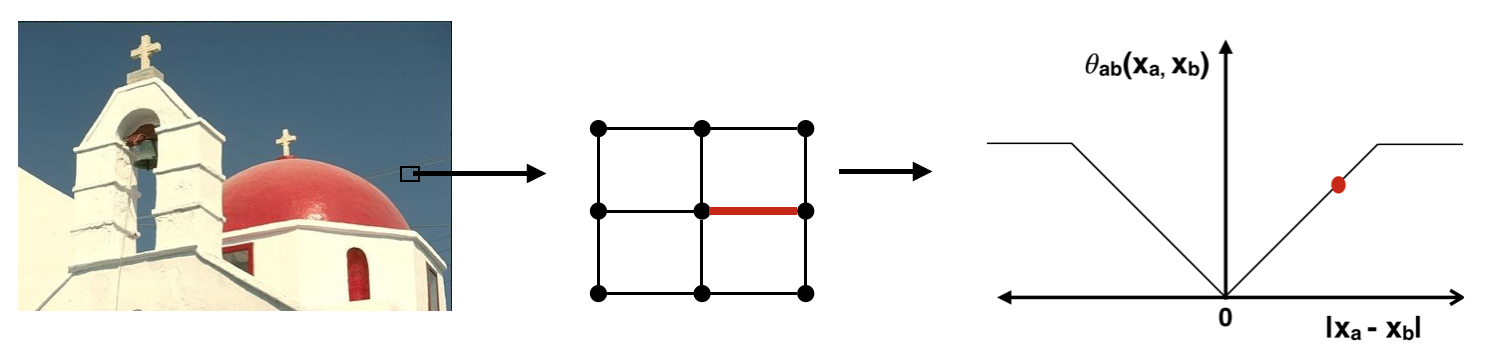
\includegraphics[scale = 0.4]{\imagePath/theoryFig/tcm} \\
	(a) Truncated convex model \\
	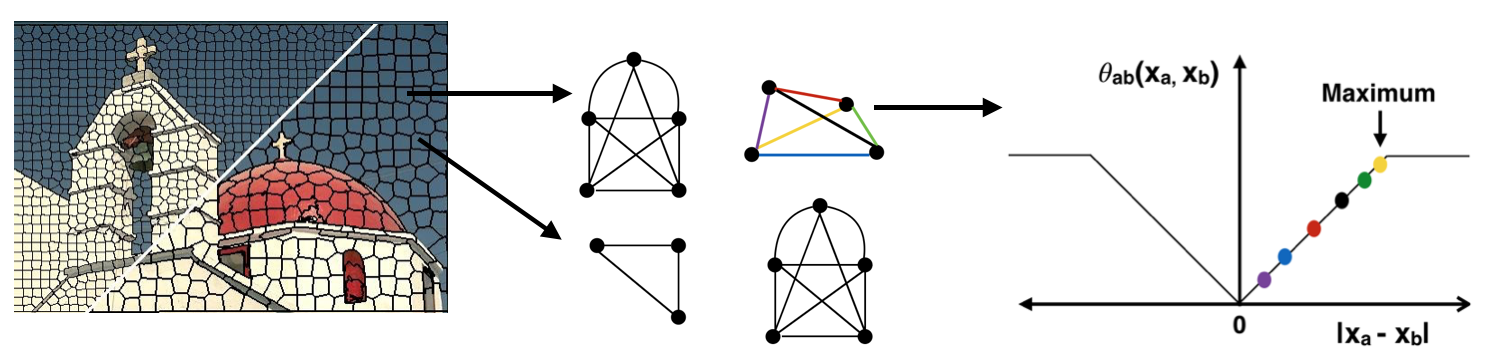
\includegraphics[scale = 0.4]{\imagePath/theoryFig/tmcm} \\ 
	(b) Truncated max-of-convex model \\
\end{tabular}
\vspace{8mm}
\mycaption{\footnotesize \em TMCM as generalization of TCM. In (a), given an image, TCM considers pairwise 4-neighborhood relationships and uses truncated convex distance function for pairwise potential. In (b), TMCM considers superpixels as cliques. The clique potential for $m$ =1 is the maximum over all the pairwise truncated convex distances.}  
\vspace{-5mm}
\label{fig:tmcm_concept}
\end{figure}


An assignment of values to all the variables is referred to as a labeling. In order to quantitatively distinguish the labelings, a TCM
specifies an energy function that consists of two types of potentials. First, a unary potential that depends on the label
of one random variable, and has no restriction on its form. Second, a pairwise potential that depends on the labels of
two neighboring random variables. The pairwise potential is proportional to the truncated convex distance between the
labels. Convex distance function encourages smoothness in the labeling, while the use of truncation allows
for discontinuities in the labeling.

Given an input, the output is obtained by minimizing the energy function of a TCM over all possible labelings. While this
is an NP-hard problem, several approximate algorithms have been proposed
in the literature~\cite{boykovpami01,chekurisoda01,guptastoc00,kolmogorovpami06,komodakisiccv07,komodakiscvpr07,kumarnips08,vekslercvpr07},
which provide accurate solutions in practice~\cite{szeliskipami08}.
In fact, there are compelling theoretical reasons to believe that linear programming relaxation based approaches~\cite{chekurisoda01,kolmogorovpami06,kumarnips08}
are the best polynomial-time algorithms that can be devised for energy minimization~\cite{manokaranstoc08}.
Of particular interest is the range expansion algorithm that combines the efficiency of
$st$-{\sc mincut} with the accuracy of linear programming~\cite{kumarnips08}.

Since we cannot reasonably expect to improve the optimization of TCM, any failure cases must be addressed by modifying the
model itself to better capture image statistics. To this end, we propose to address one of the main deficiencies of
TCM, namely, the restriction to potentials of order at most two. Specifically, we propose a natural generalization of
TCM to high-order random fields, which we refer to as {\em truncated max-of-convex models} (TMCM). 
Similar to TCM, our model places no restrictions on the unary potentials.
Furthermore, unlike TCM, it allows us to define clique potentials over an arbitrary number of random variables.
The value of the clique potential is proportional to the sum of the truncation of the $m$ largest convex distances computed over disjoint pairs
of random variables in the clique. Here, 
disjoint pairs imply that the label of no random variable is used more than once to
compute the value of the clique potential. Figure~\ref{fig:tmcm_concept} demonstrates how TMCM differs from TCM. The exact mathematical form of the TMCM energy function will be presented in section ~\ref{sec:TMCM}.
The term $m$ is a positive integer that is less than or equal to half the number of variables in the smallest clique.
Importantly, the constant of proportionality for each clique potential can depend on the input
corresponding to all the random variables in the clique. This can help capture more interesting image statistics, which in turn can lead to
a more desirable output. For example, in image
denoising, instead of using pairwise potentials that measure the difference in intensity of two neighboring pixels, we can use the variance
of intensity values over a superpixel (group of pixels with similar semantic and perceptual characteristics).

In order to enable the use of TMCMs in practice, we require an efficient and accurate energy minimization algorithm
that can compute the output for a given input. To this end, we extend the range expansion algorithm for TCM to
deal with arbitrary sized clique potentials. Our algorithm retains the desirable property of iteratively solving an $st$-{\sc mincut} problem over
an appropriate directed graph (where the number of vertices and arcs grows linearly with the number of random variables, labels and cliques). As the $st$-{\sc mincut}
problem lends itself to several fast algorithms~\cite{boykovpami04}, this makes our overall approach computationally efficient. Furthermore,
we provide strong theoretical guarantees on the quality of the solution for several special cases of interest,
which establishes its accuracy. Using synthetic and standard real
datasets, we show the benefit of high-order TMCM over pairwise TCM, as well as the advantage of our range expansion
algorithm over other $st$-{\sc mincut} based approaches.

\mysection{Related Work}
Pairwise truncated convex models (TCM) offer a natural framework to capture low-level cues for
vision problems such as image denoising, stereo correspondence, segmentation and
optical flow~\cite{szeliskipami08}.
Specifically, through the use of convex distance functions they encourage smoothness in the labeling. Smooth labelings
are desirable in low-level vision since images typically have large homogeneous regions
that correspond to a single object. At the same time, TCM
allow for discontinuities in the labeling, which is expected to occur at edge pixels between two objects.
Their use is also supported by the availability of a vast number of highly efficient and accurate energy minimization
algorithms~\cite{boykovpami01,chekurisoda01,guptastoc00,kolmogorovpami06,komodakisiccv07,komodakiscvpr07,kumarnips08,vekslercvpr07}.
However, the restriction to pairwise potentials limits their representational power.

For the past few years, there has been a growing interest in high-order models. In this work, our
focus is on models that admit efficient $st$-{\sc mincut} based solutions and provide strong theoretical guarantees on the
quality of the solution. One early work was the $P^n$ Potts model~\cite{kohlicvpr07}, which encourages label consistency
over a set of random variables. This work has extended in~\cite{kohlicvpr08}, which introduced robustness in the $P^n$ Potts model by
taking into account the number of random variables that disagreed with the majority label of a clique. Both the $P^n$ Potts
model and its robust version lend themselves to efficient optimization via the expansion algorithm~\cite{boykovpami01}, which solves
one $st$-{\sc mincut} problem at each iteration. The expansion algorithm provides multiplicative bounds~\cite{gouldcvpr09},
which measure the quality of the estimated labeling with respect to the optimal one. Our work generalizes both
the models, as well as the corresponding
expansion algorithm. Specifically, when the truncation factor of our models is set to 1, we recover the robust $P^n$ model.
Furthermore, a suitable setting of the range expansion algorithm (setting the interval length to 1) recovers the
expansion algorithm.

Delong et al.\ \cite{delongijcv12,delongcvpr10} proposed a clique potential based on label costs that can also be handled via the expansion algorithm.
However, unlike the robust $P^n$ Potts model, their model provides additive bounds that are not invariant to reparameterizations
of the energy function. This theoretical limitation is addressed by the recent work of Dokania and Kumar~\cite{dokaniaiccv15} on parsimonious
labeling. Here, the clique potentials are defined as being proportional to a diversity function of the set of unique labels present
in the clique labeling. Our work can be thought of as being complementary to parsimonious labeling. Specifically, while parsimonious labeling
is an extension of pairwise metric labeling to high-order models, our work is an extension of truncated convex models. The only
metric that also results in a truncated convex model is the truncated linear distance. As will be seen in our experiments, our
specialized range expansion algorithm provides significantly better results for truncated max-of-linear models compared to the
hierarchical graph cuts approach of~\cite{dokaniaiccv15}.

 
We note that there have been several works that deal with more general high-order potentials and design $st$-{\sc mincut} style
solutions for them. For example, Fix et al.\ \cite{fixcvpr14} use the submodular max-flow algorithm~\cite{kolmogorovdam12}, while Arora et al.\ \cite{aroracvpr14} use
generic cuts. However, the resulting algorithms are exponential in the size of the cliques, which prevents their use in applications
that require very high-order cliques (with hundreds or even thousands of random variables). A notable exception to this is the
work of Ladicky et al.\ \cite{ladickyeccv10}, who proposed a co-occurrence based clique potential whose only requirement is that it should
increase monotonically with the set of unique labels represent in the clique labeling. However, the use of such a general
clique potential still results in an inaccurate energy minimization algorithm, as demonstrated in our experimental comparison. 

\mysection{Truncated Convex Models}

Before describing our model, we briefly review standard pairwise TCM, which will help set up the
necessary notation. A TCM is a random field defined by a set of discrete random variables
${\bf X} = \{X_a, a \in {\cal V}\}$, and a neighborhood relationship ${\cal E}$ over them (that is, $X_a$ and $X_b$ are neighboring random
variables if $(a,b) \in {\cal E}$).
Each random variable can take a value from a finite label set ${\bf L}$, which
is assumed to be ordered so as to enable the use of convex distance functions. Without loss of generality, we define
${\cal V} = \{1,2,\cdots,n\}$ and ${\bf L} = \{1,2,\cdots,h\}$.

A labeling ${\bf x} \in {\bf L}^n$ refers to an assignment of values to all the random variables.
In order to quantitatively distinguish the $h^n$ possible labelings of the random variables, a TCM defines an energy function that consists of
two types of potentials. First, the unary potentials $\theta_a(x_a)$ that depend on the label $x_a$ of one random variable $X_a$. Second,
the pairwise potentials $\theta_{ab}(x_a,x_b)$ that depend on the labels $x_a$ and $x_b$ of a pair of neighboring random variables
$(X_a,X_b)$. The form of the unary potentials is unrestricted. However, the pairwise potentials
are defined using a truncated convex distance function over the label set.

In order to provide a formal specification of the pairwise potentials, we require some definitions. We denote a convex distance function by
$d: \mathbb{Z} \rightarrow \mathbb{R}$ (where $\mathbb{Z}$ is the set of integers and $\mathbb{R}$ is the set of real numbers).
Popular examples of convex distance functions include the linear distance (that is, $d(y) = |y|$) and the quadratic
distance function (that is, $d(y) = y^2$).

Given two labels $i,j \in {\bf L}$, we can use a convex function $d(\cdot)$ to measure the distance between them as $d(i-j)$. The ability of convex distance functions to encourage smoothness makes them highly suited for low-level vision problems as images tend to
consist of large homogeneous regions. However, images
also naturally contain some discontinuities (for example, the intensity values of edge pixels differ greatly). In order to prevent
the overpenalization of the discontinuities, it is common practice to use a truncated convex distance function over the
label set~\cite{boykovpami01,kumarnips08,vekslercvpr07}.
Formally, a truncated convex function is defined as $\min\{d(\cdot),M\}$, where $M$ is the truncation factor. Using a truncated
convex function, we define the pairwise potential as $\theta_{ab}(x_a,x_b) = \omega_{ab}\min\{d(x_a-x_b),M\}$, where $\omega_{ab}$ is a
(data-dependent) non-negative constant of proportionality. Note that M must be chosen appropriately - very small M would result in uniform object patches with insufficient details, while large M would blur object boundaries.

To summarize, a TCM specifies an energy function $E(\cdot)$ over the labelings ${\bf x} \in {\bf L}^n$ as follows:
\begin{equation}
\small E({\bf x}) = \sum_{a \in {\cal V}} \theta_a(x_a) + \sum_{(a,b) \in {\cal E}} \omega_{ab}\min\{d(x_a-x_b),M\}.
\end{equation}
The unary potentials are arbitrary, the edge weights $\omega_{ab}$ are non-negative, $d(\cdot)$ is a convex function and
$M \geq 0$ is the truncation factor.
Given an input (which provides the values of the unary potentials and the edge weights), the desired output is obtained by solving the following
optimization problem: $\min_{{\bf x} \in {\bf L}^n} E({\bf x})$. While this optimization problem is NP-hard, we can obtain an accurate approximate
solution by using the efficient range expansion algorithm~\cite{kumarnips08}, as well as several
other approaches based on $st$-{\sc mincut}~\cite{boykovpami01,guptastoc00,komodakiscvpr07,vekslercvpr07}
and linear programming~\cite{chekurisoda01,kolmogorovpami06,komodakisiccv07}.

\mysection{Truncated Max-of-Convex Models}
\label{sec:TMCM}

Our aim is to obtain a natural generalization of TCM to high-order random fields, which define potentials over random variables that
form a clique (where all the random variables in a clique are neighbors of each other). Importantly, we do not want to place any
restriction on the size of the clique. We propose
to use the {\em sum of the truncation of the $m$ largest convex distances over disjoint pairs of random variables} that belong to the clique. We first formally specify the
form of our high-order clique potentials. This will allow us to subsequently discuss its advantages in modeling low-level vision applications.

\myparagraph{\bf Truncated Max-of-Convex Potentials.} Consider a high-order clique consisting of the random variables ${\bf X}_{\bf c} = \{X_a, a \in {\bf c} \subseteq {\cal V}\}$.
We denote a labeling of the clique as ${\bf x}_{\bf c} \in {\bf L}^{c}$, where we have used the shorthand $c = |{\bf c}|$ to denote the size of the clique.
In order to specify the value of the clique potential for the labeling ${\bf x}_{\bf c}$ we
require a sorted list of the (not necessarily unique) labels present in ${\bf x}_{\bf c}$. We denote this sorted list by ${\bf p}({\bf x}_{\bf c})$
and access its $i$-th element as $p_i({\bf x}_{\bf c})$. For example, consider a clique consisting of random variables ${\bf X}_{\bf c} = \{X_1,X_2,X_3,X_4,X_5,X_6\}$.
If the number of labels $h = 10$, then one of the putative labelings of the clique is ${\bf x}_{\bf c} = \{3,2,1,4,1,3\}$ (that is, $X_1$ takes the value $3$,
$X_2$ takes the value $2$ and so on). For this labeling, ${\bf p}({\bf x}_{\bf c}) = \{1,1,2,3,3,4\}$. The value of $p_1({\bf x}_{\bf c})$ and
$p_2({\bf x}_{\bf c})$ is $1$, the value of $p_3({\bf x}_{\bf c})$ is $2$ and so on. Given a convex function $d(\cdot)$, a truncation factor $M$ and an integer
$m \in [0,\floor{c/2}]$, the clique potential $\theta_{\bf c}(\cdot)$ is defined as

\begin{equation}
\small \theta_{\bf c}({\bf x}_{\bf c}) = \omega_{\bf c} \sum_{i=1}^m \min\{d(p_i({\bf x}_{\bf c})-p_{c-i+1}({\bf x}_{\bf c})),M\}.
\label{eq:maxPotential}
\end{equation}

Here, $\omega_{\bf c} \geq 0$ is the clique weight that does not depend on the labeling. However, it can be chosen based on the observed data - for instance, we may want to assign small weights to cliques with large variance of intensity, disparity, etc. The term inside the summation is the truncated
value of the $i$-th largest distance between the labels of all pairs of random variables within the clique, subject to the constraint that the label of no random
variable is used more than once in the computation of the clique potential value. In other words, our clique potential is proportional to the
sum of the truncation of the $m$ largest convex distance functions over disjoint pairs of random variables. 

%In the remaining part of this section, we will analyze the advantages of our high-order potentials from a modeling point of view. The next
%section will demonstrate their computational advantage by generalizing the efficient
%range expansion algorithm to accurately minimize energy functions that consist of arbitrary unary potentials and high-order
%truncated max-of-convex potentials.

Table~\ref{table:cliqueExample} demonstrates how TMCM ensures smooth labelings, prevents overpenalization of discontinuities (desirable at object boundaries) and provides robustness to erroneous clique defintions which may happen if division of image into superpixels is not perfect. As an example, consider labeling \{1, 1, 1, 1, 2, 2\} and $M$ = 3, $m$ = 3, $\bf\omega_c$ = 1 as in pair (a). Using equation~\ref{eq:maxPotential}, $\theta_{\bf c}({\bf x}_{\bf c})$ = min(6-1, 3) + min(5 - 2, 6) + min(4 - 3, 3) = 3 + 3 + 1 = 7.
\vspace{-2mm}

%\begin{table}[h!]
%%\begin{center}
%\fcapside[\FBwidth]
%{\mycaption{\small \em Clique potential value $\theta_{\bf c}({\bf x}_{\bf c})$ defined by a linear function with $M$ = 3 and $\bf{\omega_c}$ = 1 for various
%		values of $m$. Since clique size is 6, $0 \leq m \leq 3$. Pair (a)
%		demonstrates why taking the largest convex distances favors smoothness. (b) demonstrates how truncation prevents overpenalizing
%		discontinuities. (c) demonstrates how using $m > 1$ can provide some degree of robustness to errors in the definitions of the cliques.
%}
%\label{table:cliqueExample}
%}	
%{
%\begin{tabular}{|r|c|c|c|}
%\hline
%Labeling & $m=1$ & $m=2$ & $m=3$ \\
%\hline
%(a) \{1,1,1,1,2,2\} & 1 & 2 & 2 \\
%\{1,2,3,4,5,6\} & 3 & 6 & 7 \\
%\hline
%(b) \{1,1,1,9,9,9\} & 3 & 6 & 9 \\
%\{1,1,1,8,8,9\} & 3 & 6 & 9 \\
%\hline
%(c) \{1,1,1,1,1,7\} & 3 & 3 & 3 \\
%\{1,1,1,2,3,4\} & 3 & 5 & 6 \\
%\hline
%\end{tabular}
%}
%%\end{center}
%\end{table}

\begin{table}[h!]
%\begin{center}
%\fcapside[\FBwidth]
{\mycaption{\footnotesize \em Clique potential value $\theta_{\bf c}({\bf x}_{\bf c})$ defined by a linear function with $M$ = 3 and $\bf{\omega_c}$ = 1 for various
		values of $m$. Since clique size is 6, $0 \leq m \leq 3$. Pair (a)
		demonstrates why taking the largest convex distances favors smoothness. (b) demonstrates how truncation prevents overpenalization of
		discontinuities. (c) demonstrates how using $m > 1$ can provide some degree of robustness to errors in the definitions of the cliques.
}
\label{table:cliqueExample}
}	
{
\begin{tabular}{|r|c|c|c|}
\hline
Labeling & $m=1$ & $m=2$ & $m=3$ \\
\hline
(a) \{1,1,1,1,2,2\} & 1 & 2 & 2 \\
\{1,2,3,4,5,6\} & 3 & 6 & 7 \\
\hline
(b) \{1,1,1,9,9,9\} & 3 & 6 & 9 \\
\{1,1,1,8,8,9\} & 3 & 6 & 9 \\
\hline
(c) \{1,1,1,1,1,7\} & 3 & 3 & 3 \\
\{1,1,1,2,3,4\} & 3 & 5 & 6 \\
\hline
\end{tabular}
}
%\end{center}
\end{table}



To summarize, a TMCM specifies the following energy function $E(\cdot)$ over the labelings ${\bf x} \in {\bf L}^n$:
\begin{equation}
\small E({\bf x}) = \sum_{a \in {\cal V}} \theta_a(x_a) + \sum_{{\bf c} \in {\cal C}} \theta_{\bf c}({\bf x}_{\bf c}).
\end{equation}
Here, the unary potentials $\theta_a(\cdot)$ are arbitrary, the clique potentials $\theta_{\bf c}(\cdot)$ are as defined in
equation~(\ref{eq:maxPotential}), and ${\cal C}$ refers to the set of all cliques in the random field.  Given an input, the
desired output is obtained by solving the following optimization problem: $\min_{{\bf x} \in {\bf L}^n} E({\bf x})$. Note that TMCM is a generalization of the $P^n$ Potts model~\cite{kohlicvpr07} ($m$ = 1, $M$ = 1) as well as its robust version~\cite{kohlicvpr08} ($m > $  1, $M$ = 1). Furthermore, it is complementary to the recently proposed parsimonious labeling, which generalizes metric labeling.
Henceforth, we assume the
unary potentials are non-negative. Note that this assumption is not restrictive as we can always add a constant to the unary potentials
of a random variable. This modification would only result in the energy of all labelings changing by the same constant. As will be seen
shortly, our algorithm as well as its theoretical guarantees are invariant to such changes in the energy function.

\mysection{Optimization via Range Expansion}
As TMCMs are a generalization of TCM, it follows that the corresponding energy
minimization problem is NP-hard. However, we show that the efficient and accurate
range expansion algorithm can be extended to handle this more general class
of energy functions. Due to space limitations, we only provide an overview of our
approach. The algorithm is described in detail in the supplementary
material, which also contains the proofs of our propositions.

The range expansion algorithm is an iterative move-making method, which starts with an initial labeling
${\bf x}^0$. At each iteration, given the current labeling $\hat{\bf x}$ it attempts to move to a labeling with lower energy value
by allowing each random variable $X_a$ to either retain its old label $\hat{x}_a$ or choose a new label from an
interval ${\bf I} = \{s,\cdots,l\}$ of length $h' = l-s+1$. In other words, a new labeling is chosen by solving the
following optimization problem:
\begin{eqnarray}
{\bf x}' = && \argmin_{\bf x} E({\bf x}), \nonumber \\
&& \mbox{s.t. } x_a \in {\bf I} \cup \{\hat{x}_a\}, \forall a \in {\cal V}.
\label{eq:rangeMove}
\end{eqnarray}
At each iteration, the range expansion algorithm chooses a new interval ${\bf I}$ of length $h'$. The algorithm converges
when the energy of the labeling cannot be reduced further for any choice of the interval. Algorithm~\ref{algo:rangeExpansion} gives an overview of the range expansion algorithm for TMCM.

The main challenge we face is that problem~(\ref{eq:rangeMove}) itself may be NP-hard. Indeed, when $h'=h$,
problem~(\ref{eq:rangeMove}) is equivalent to the original energy minimization problem. To alleviate this difficulty, we
propose an $st$-{\sc mincut} based approximate solution to the above problem. In other words, we construct a directed graph
whose cuts encode the putative labelings of problem~(\ref{eq:rangeMove}). We obtain an approximate solution ${\bf x}'$ by
computing the $st$-{\sc mincut}. The graph construction for a given current labeling $\hat{\bf x}$ and
an interval ${\bf I}$ of some arbitrary length $h'$ is described in the next subsection. Subsection~\ref{subsec:bounds}
provides strong theoretical guarantees for various special cases of interest. This serves two purposes: (i) it establishes
the accuracy of range expansion for TMCM; and (ii) it helps identify the optimal value of the interval length parameter.
\vspace{-2mm}
\begin{algorithm}
\small
\caption{The range expansion algorithm for TMCM.}
\begin{algorithmic}[1]
\INPUT Energy function $E(\cdot)$, initial labeling ${\bf x}^0$, interval length $L$.
\STATE Initialize the output labeling $\hat{\bf x} = {\bf x}^0$.
\REPEAT
\FORALL{$i_m \in [-L+2,h]$}
\STATE Define an interval of labels ${\bf I} = \{f,\cdots,l\}$ where $f = \max\{i_m,1\}$ and
$l = \min\{i_m+L-1,h\}$.
\STATE Obtain a new labeling ${\bf x}'$ by solving the following optimization problem:
\begin{eqnarray}
{\bf x}' = && \argmin_{\bf x} E({\bf x}), \nonumber \\
&& \mbox{s.t. } x_a \in {\bf I} \cup \{\hat{x}_a\}, \forall a \in {\cal V}.
\label{eq:rangeMove}
\end{eqnarray}
\IF{$E(\hat{\bf x}) > E({\bf x}')$}
\STATE Update $\hat{\bf x} = {\bf x}'$.
\ENDIF
\ENDFOR
\UNTIL The labeling does not change for any value of $i_m$.
\OUTPUT The labeling $\hat{\bf x}$.
\end{algorithmic}
\label{algo:rangeExpansion}
\end{algorithm}

\mysubsection{Graph Construction}
\label{subsec:graph}
Our problem is to minimize the energy function $E(\cdot)$ over all possible labelings that allow each random variable $X_a$ to either
retain its current label $\hat{x}_a$ or choose a label from the interval ${\bf I} = \{s,\cdots,l\}$.
To this end, we convert it into an equivalent $st$-{\sc mincut} problem over a directed graph, which can be solved efficiently if all arc capacities are non-negative~\cite{boykovpami04}.

We construct a directed graph over the set of vertices $\{s,t\} \cup {\bf V} \cup {\bf U} \cup {\bf W}$. The set of vertices ${\bf V}$ model the random variables
${\bf X}$. Specifically,
for each random variable $X_a$ we define $h'=l-s+1$ vertices $V^a_i$ where $i \in \{1,\cdots,h'\}$.
The sets ${\bf U}$ and ${\bf W}$ represent {\em auxiliary}
vertices, whose role in the graph construction will be explained later when we consider representing the high-order clique potentials. We also define a set of
arcs over the vertices, where each arc has a non-negative capacity.
We would like to assign arc capacities such that the $st$-cuts of the directed graph satisfy two properties. First, all the $st$-cuts with a finite capacity
should include exactly one arc from the set $(s,V^a_1) \cup \{(V^a_i,V^a_{i+1}), i=1,\cdots,h'-1\} \cup (V^a_{h'},t)$
for each random variable $X_a$. This property would allow us to define a labeling ${\bf x}$ such that
\begin{equation}
\small x_a = \left\{
\begin{array}{cl}
\hat{x}_a & \mbox{if the cut includes the arc } (s,V^a_1) \\
s+i-1 & \mbox{if the cut includes the arc } (V^a_i,V^a_{i+1}) \\
l & \mbox{if the cut includes the arc } (V^a_{h'},t). \\
\end{array}
\right.
\label{eq:labeling}
\end{equation}

Second, we would like the energy of the labeling {\bf x} defined above to be as close as possible to the capacity of the $st$-cut. This will allow
us to obtain an accurate approximate solution ${\bf x}'$ for problem~(\ref{eq:rangeMove}) by finding the $st$-{\sc mincut}.
We now specify the arcs and their capacities such that they
satisfy the above two properties. We consider two cases: (i) arcs that represent the unary potentials; and (ii) arcs that represent the high-order clique potentials.

\begin{figure*}
\centerline{
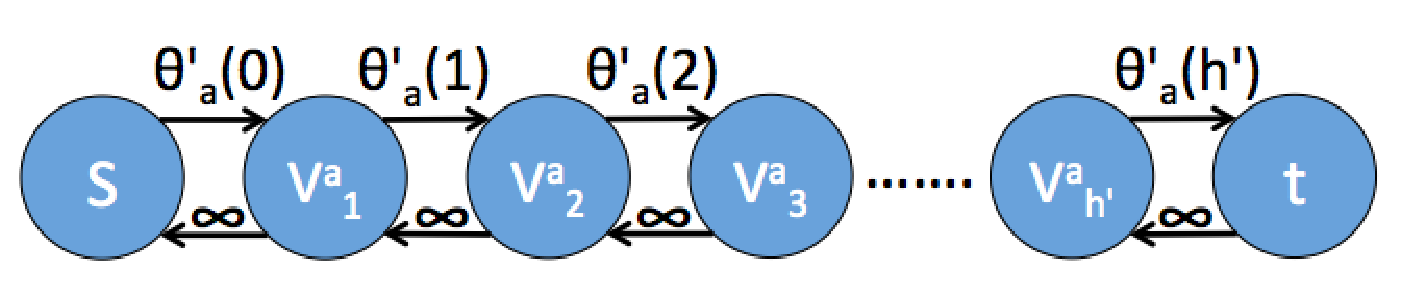
\psfig{file=./\imagePath/theoryFig/unary_alt.eps,width=0.6\textwidth}
}
\vspace{3mm}
\mycaption{\footnotesize \em Arcs and their capacities for representing the unary potentials for the random variable $X_a$. According to the labeling defined
in equation~(\ref{eq:labeling}), if $x_a = \hat{x}_a$, then the arc $(s,V^a_1)$ will be cut, which will contribute exactly
$\theta_a(\hat{x}_a)$ to the capacity of the cut.
If $x_a = s+i-1$ where $i \in \{1,\cdots,h'-1\}$, then the arc $(V^a_i,V^a_{i+1})$ will be cut, which will contribute
exactly $\theta_a(s+i-1)$ to the capacity of the cut. If $x_a = l$, then the arc $(V^a_{h'},t)$ will be cut, which will contribute exactly
$\theta_a(l)$ to the capacity of the cut. The arcs with infinite capacity ensure that exactly one of the arcs from the set
$(s,V^a_1) \cup \{(V^a_i,V^a_{i+1}), i=1,\cdots,h'-1\} \cup (V^a_{h'},t)$ will be part of an $st$-cut with finite capacity,
which will guarantee that we are able to obtain a valid labeling.
}
\label{fig:unary}
\end{figure*}

\myparagraph{\bf Representing Unary Potentials.}
We will represent the unary potential
of $X_a$ using the arcs specified in Figure~\ref{fig:unary}. Since all the unary potentials are non-negative, it follows that the arc
capacities in Figure~\ref{fig:unary} are also non-negative.

\begin{figure*}[t]
\centering
\psfig{file=./\imagePath/theoryFig/clique1.eps,width=0.30\textwidth}
\hspace{3cm}
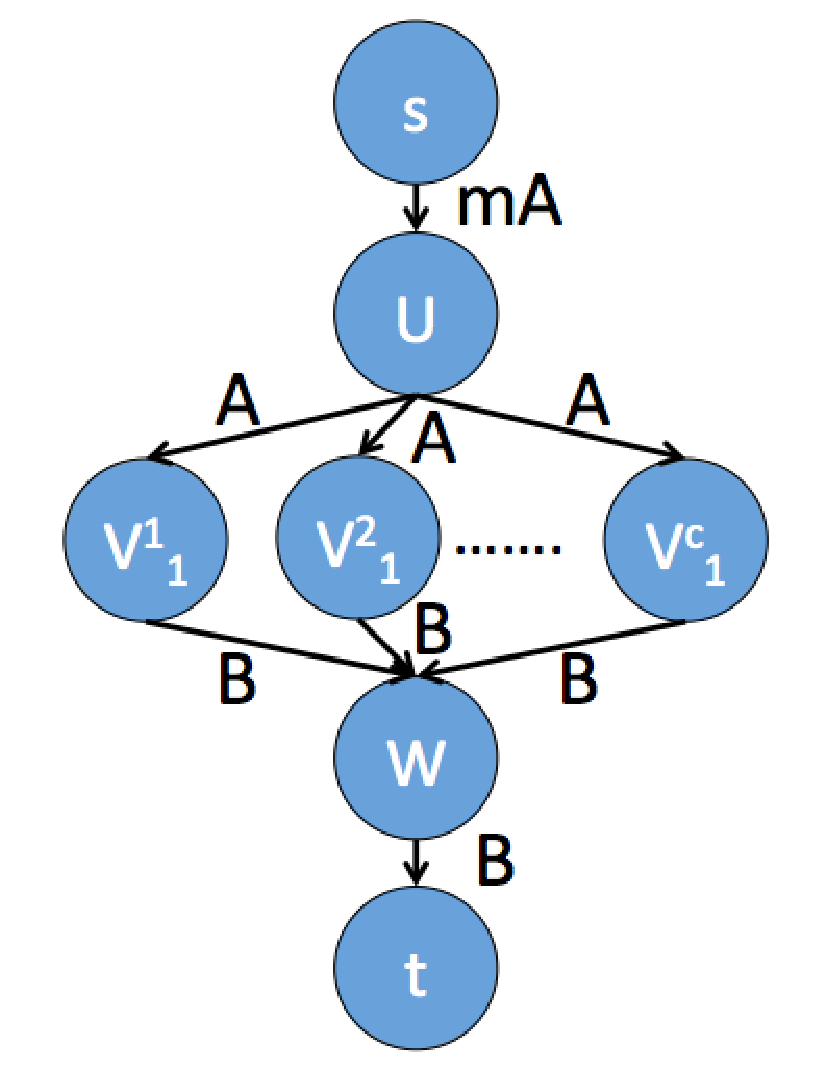
\psfig{file=./\imagePath/theoryFig/clique2.eps,width=0.30\textwidth}
\vspace{2mm}
\mycaption{\footnotesize \em Arcs used to represent the high-order potentials for the clique ${\bf X}_{\bf c} = \{X_1,X_2,\cdots,X_c\}$. {\bf Left.}
The term $r_{ij}$ is defined in equation~(\ref{eq:convexCapacity}). The arcs 
represent the sum of the $m$ maximum convex distance functions over disjoint pairs of random variables when no random variable retains
its old label. These arcs are specified only for $i \leq j$ and
when either one or both of $i$ and $j$ are not equal to 1. {\bf Right.} The terms $A$ and $B$ are defined in equation~(\ref{eq:submodCapacity}).
The arcs represent an overestimation of the clique potential for the case where some or all the random variables retain their old label.
}
\label{fig:clique}
\end{figure*}

\myparagraph{\bf Representing Clique Potentials.}
Consider a set of random variables ${\bf X}_{\bf c}$ that are used to define a high-order clique potential. Without loss of generality, we assume
${\bf X}_{\bf c} = \{X_1,X_2,\cdots,X_c\}$. In order to represent the potential value for a putative labeling ${\bf x}_{\bf c}$ of the clique, we
introduce two types of arcs, which are depicted in Figure~\ref{fig:clique}. For the arcs shown in Figure~\ref{fig:clique} (left), the capacities are
specified using the term $r_{ij}$ that is defined as follows:
\begin{equation}
\small r_{ij} = 
\begin{cases}
\omega_{\bf c}\frac{\overline{d}(i,j)}{2} & \text{if } i = j\\
\omega_{\bf c}\overline{d}(i,j)   & \text{otherwise.}
\end{cases}
\label{eq:convexCapacity}
\end{equation}
Here, the term $\overline{d}(i,j) = d(i-j+1) + d(i-j-1) - 2d(i-j) \geq 0$ since $d(\cdot)$ is convex, and
$\omega_{\bf c} \geq 0$ by definition. It follows that $r_{ij} \geq 0$ for all $i,j \in \{1,\cdots,h'\}$. 
For the arcs shown in Figure~\ref{fig:clique} (right), the capacities are specified using the terms $A$ and $B$ that are defined as follows:
\begin{equation}
\small A = \omega_{\bf c}M, B = \left(\omega_{\bf c}M-\frac{\theta_{\bf c}(\hat{\bf x}_{\bf c})}{m}\right).
\label{eq:submodCapacity}
\end{equation}
Since $M \geq 0$, and $\theta_{\bf c}(\hat{\bf x}_{\bf c}) \leq \omega_{\bf c}mM$ due to truncation, it follows that $A, B \geq 0$.


\mysubsection{Multiplicative Bounds}
\label{subsec:bounds}
Similar to the case of pairwise TCM, we establish the accuracy of the range expansion algorithm
by providing strong multiplicative bounds for special cases of TMCM that are very useful in practice. The multiplicative bounds also serve to identify the best value
of the interval length parameter $h'$.

\begin{proposition}
\label{prop:linearBound}
The range expansion algorithm with $h' = M$ has a multiplicative bound of $O(C)$ for truncated max-of-linear model when $m=1$. The
term $C$ equals the size of the largest clique. Hence, if ${\bf x}^*$ is a labeling with
minimum energy and $\hat{\bf x}$ is the labeling estimated by range expansion algorithm then
\begin{equation}
\small
\sum_{a \in {\cal V}} \theta_a(\hat{x}_a) + \sum_{{\bf c} \in {\cal C}} \theta_{\bf c}(\hat{\bf x}_{\bf c}) \leq \nonumber 
\sum_{a \in {\cal V}} \theta_a({x}^*_a) + O(C) \sum_{{\bf c} \in {\cal C}} \theta_{\bf c}({\bf x}^*_{\bf c}).
\label{eq:linear_bound}
\end{equation}
The above inequality holds for arbitrary set of unary potentials and non-negative clique weights.
\end{proposition}
Note that the bound of the move making algorithm for parsimonious labeling (which is our baseline) is $\left(\frac{r}{r-1}\right) (|\mathcal{L}| - 1) O(log|\mathcal{L}|)min(\mathcal{M}, |\mathcal{L}|)$ where $\mathcal{M}$ is the size of the largest clique and $|\mathcal{L}|$ is the number of labels~\cite{dokaniaiccv15}. Our algorithm gives a better bound of ($O(C)$) and does not depend on the number of labels.

\begin{proposition}
\label{prop:quadraticBound}
The range expansion algorithm with $h' = \sqrt{M}$ has a multiplicative bound of $O(C\sqrt{M})$ for the truncated max-of-quadratic model when $m=1$.
\end{proposition}
The proofs for the above two propositions as well as the multiplicative bounds for general values
of $m$ are provided in the supplementary material.

\mysection{Experiments} 

To demonstrate the efficacy of our algorithm, we test it on both synthetic and real data. We used the parsimonious labeling algorithm of Dokania \textit{et al.}~\cite{dokaniaiccv15} and the move-making algorithm for the co-occurrence based energy function of Ladicky \textit{et al.}~\cite{ladickyeccv10} as baselines. For comparison, we restrict ourselves to max-of-linear models and $m$ = 1, as the available code for the baselines can only handle this special case. For completeness, we will report the results of our range expansion algorithm for other cases of TMCM as well.

\mysubsection{Synthetic Data}
\vspace{2mm}

\begin{figure*}[t]
\centerline{
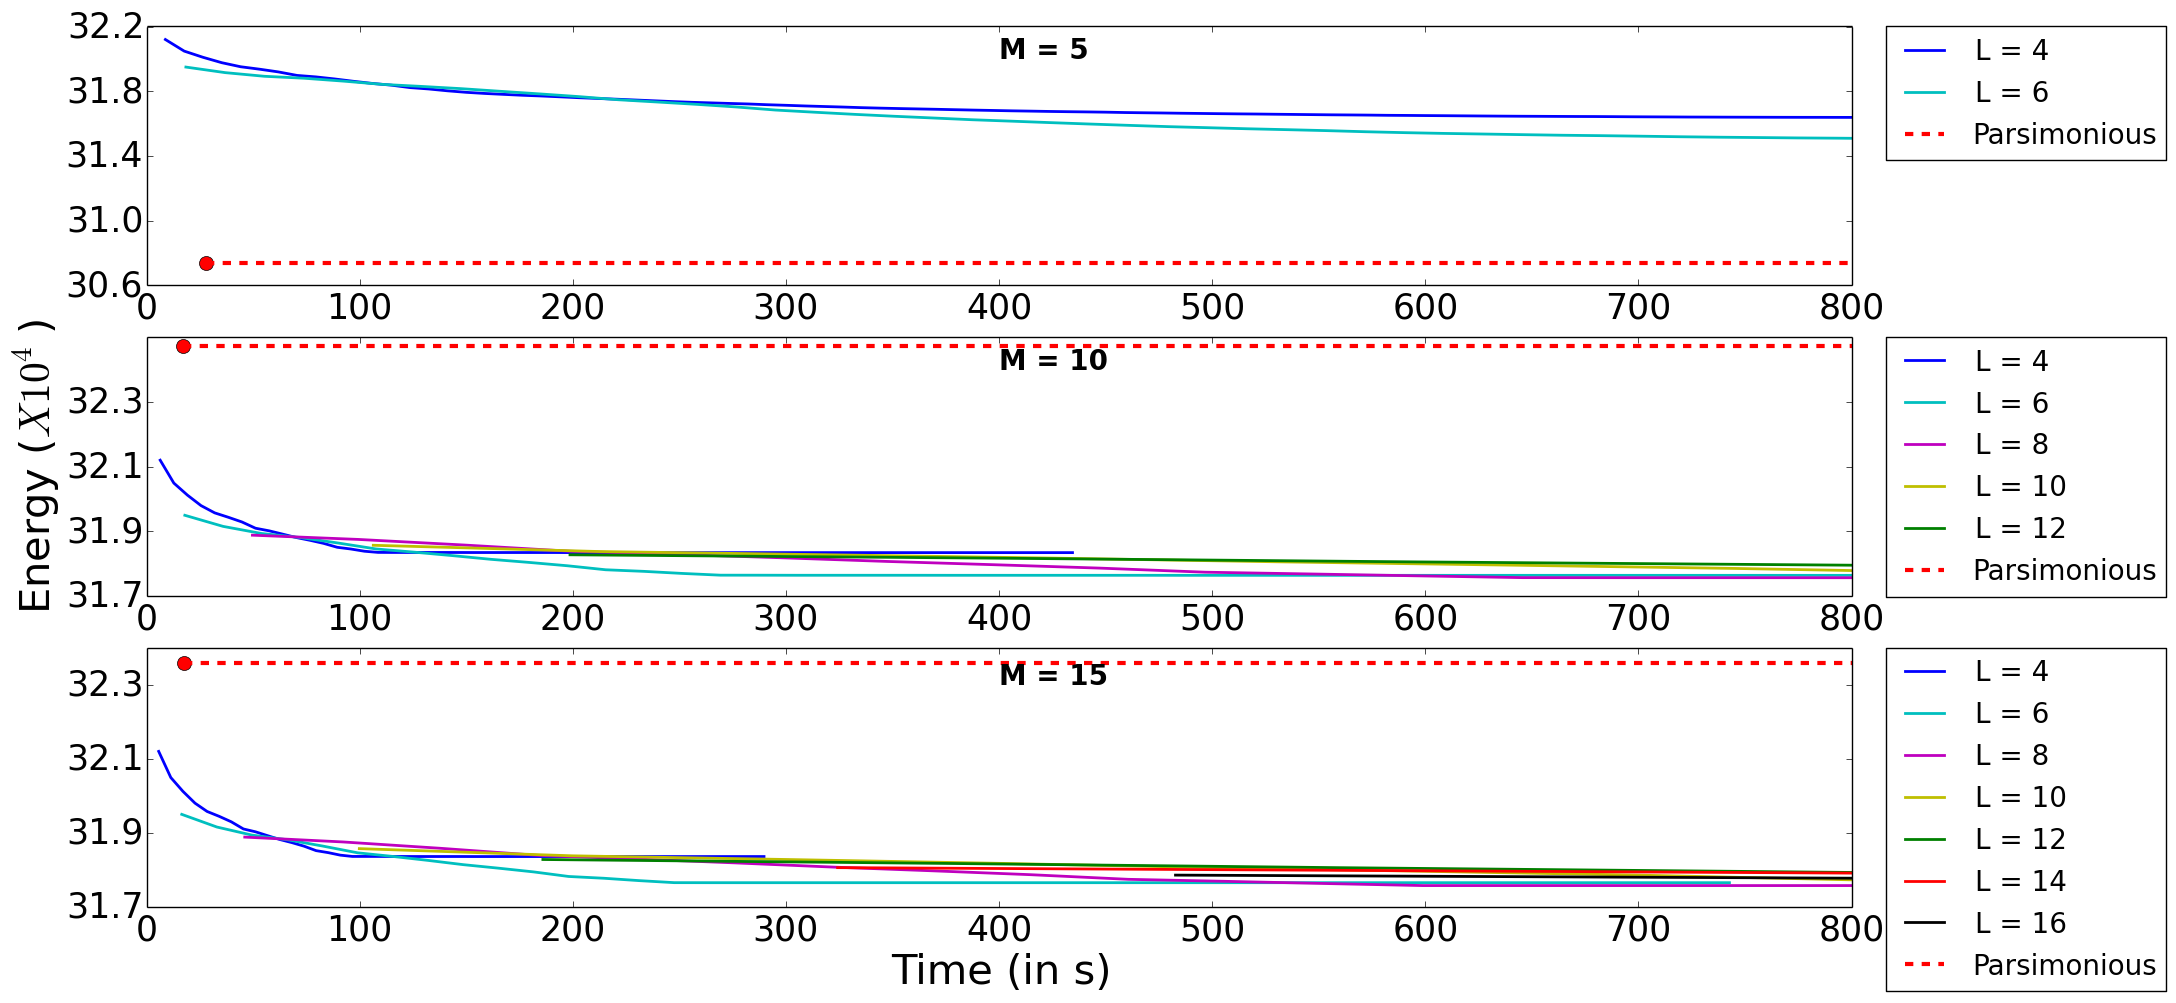
\includegraphics[keepaspectratio = true, width =0.9\textwidth]{\imagePath/synthetic_results/linear_w5}
}
\vspace{3mm}
\mycaption{\footnotesize \em Results for synthetic data using truncated linear distance function. The plots show the variation of energy versus time, averaged over 50 lattices using $\omega_c = 5$. We use truncation factors as $M$ = 5, 10 and 15  and $m$ = 1, and for each we vary interval lengths for our algorithm. Parsimonious labeling performs well for $M$ = 5, but our approach outperforms for higher values of $M$. Red dot indicates convergence of parsimonious labeling and dotted line indicates extrapolation.}
\label{fig:max-of-linear_synthetic}
\end{figure*}

\begin{figure*}[t]
\centerline{
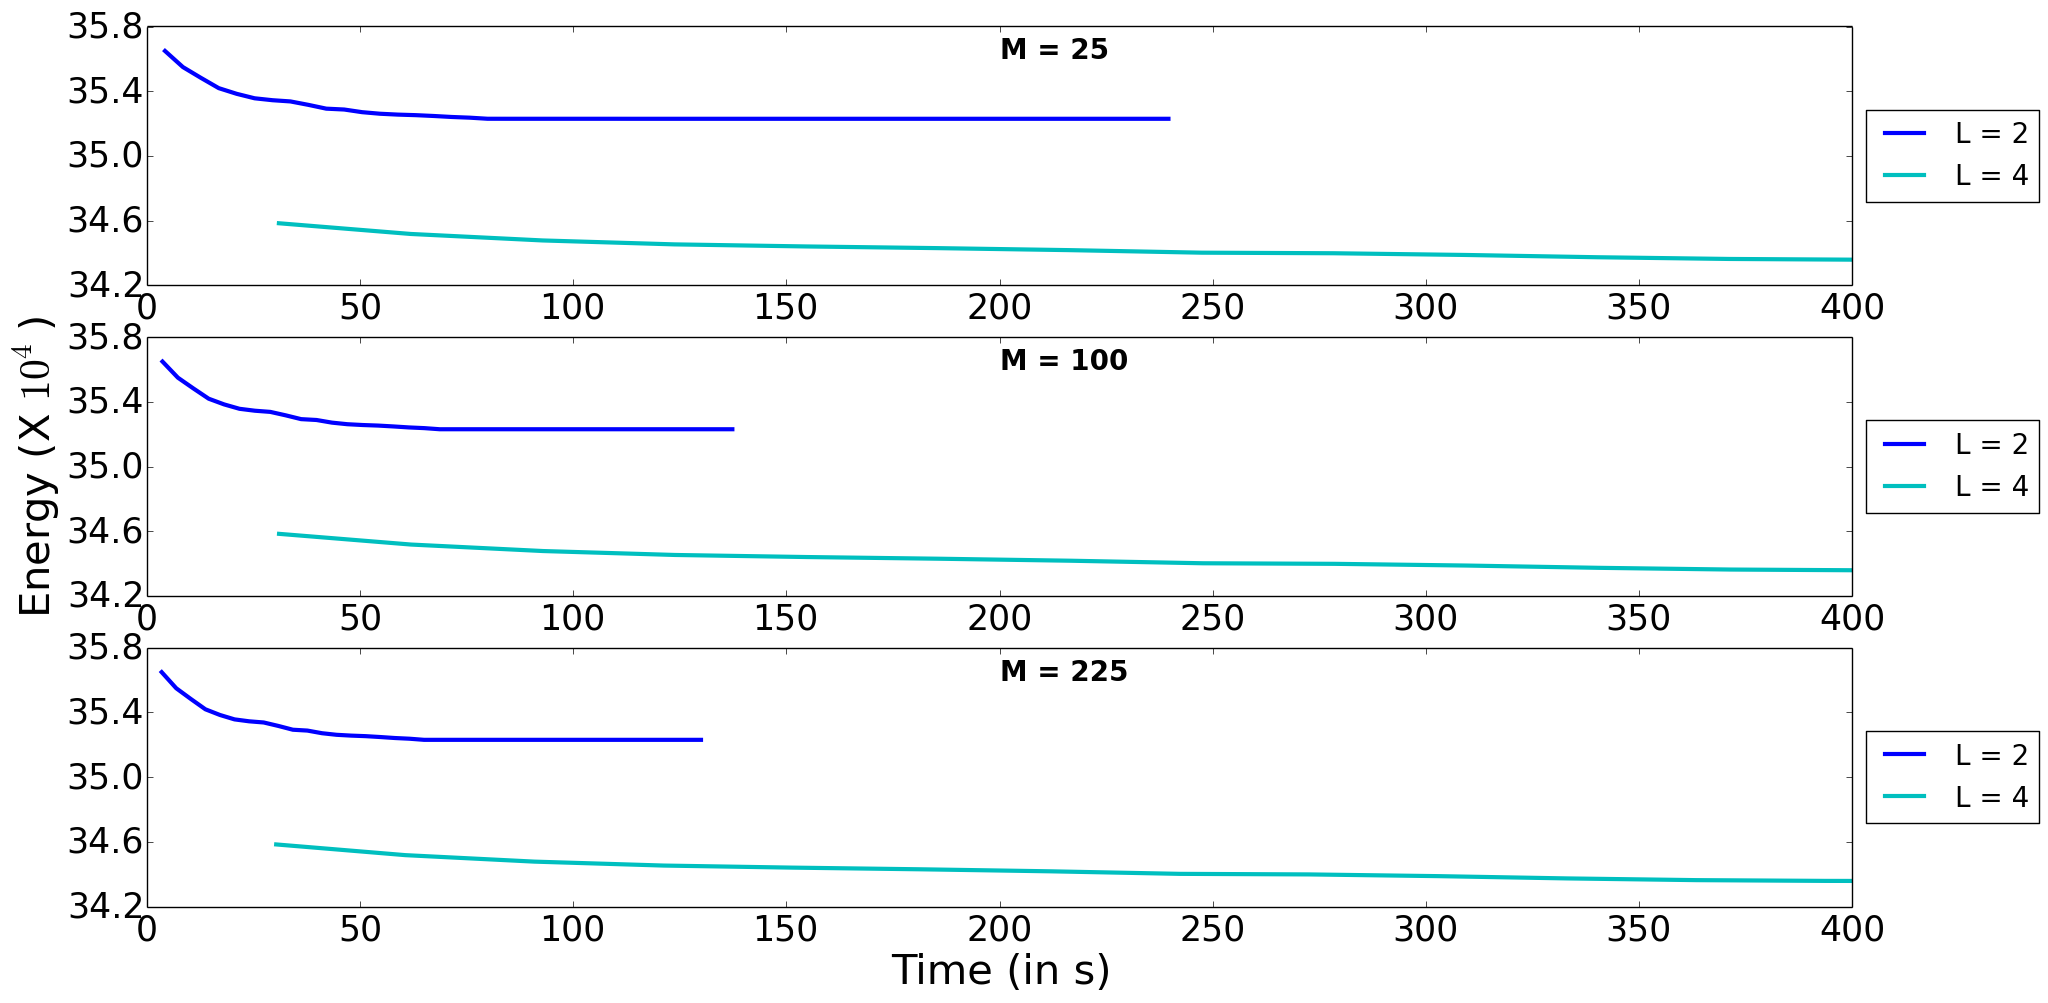
\includegraphics[keepaspectratio = true, width = 0.9\textwidth]{\imagePath/synthetic_results/quadratic_w3}
}
\vspace{3mm}
\mycaption{\footnotesize \em Results for synthetic data using truncated quadratic distance function. The plots show the variation of energy versus time, averaged over 50 lattices using $\omega_c = 3$. We use $M$ = 25, 100 and 225, and for each we vary interval lengths for our algorithm.}
\label{fig:max-of-quadratic_synthetic}
\end{figure*}

\myparagraph{\bf Data.} We generate lattices of size 100 $\times$ 100, where each lattice point represents a variable taking one of 20 labels. The cliques are defined as all 10 $\times$ 10 subwindows. The unary potentials are uniformly sampled in the range [1, 100]. The truncation factors for linear case are $M \in \{5, 10, 15\}$ and for quadratic case $M \in \{25, 100, 225\}$. In each energy function, all cliques were assumed to have the same clique weight, being 5 for linear model and 3 for quadratic model. $m$ varies in the range $\{1, 3, 5\}$. Results for other clique weights are shown in the supplementary material.

\myparagraph{\bf Method.} For each energy function obtained by a particular setting of the above parameters, we vary the interval length up to $M$ + 1. We run~\cite{dokaniaiccv15} and~\cite{ladickyeccv10} only for linear distance function and $m$ = 1. The experiments are repeated for 50 randomly generated unaries for linear and quadratic cases. 

\myparagraph{\bf Results.} The plots in Figure~\ref{fig:max-of-linear_synthetic} show the average energy as a function of average time for our algorithm and the baselines for each parameter setting for max-of-linear models. The average final energy for the co-occurrence algorithm lies outside the upper range of our plot (see supplementary material for plot including co-occurrence value). Our algorithm gives lower energy solutions than parsimonious labeling method except when the truncation factor is low ($M$ = 5). This is expected as parsimonious labeling approximates a metric using a Potts model, which is accurate for smaller values of $M$. Both the baselines converge faster than our method. In practice, intervals smaller than the optimum size give almost equally good results and converge faster. Figure~\ref{fig:max-of-quadratic_synthetic} shows the plots for max-of-quadratic cases.

\mysubsection{Real Data}

We present results on the two problems of image inpainting and denoising, and stereo matching. These enable us to visually infer the quality of our solutions. We use the energy of final labeling and convergence time as the evaluation criteria. 

\mysubsubsection{Image Inpainting and Denoising}

\begin{figure}[t]
	\centering
\begin{tabular}{ccccc}
	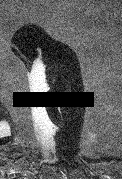
\includegraphics[scale = 0.50]{\imagePath/inpainting_results/penguin-input} &
	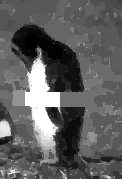
\includegraphics[scale = 0.50]{\imagePath/inpainting_results/penguin_COOC_w40_M40} &
	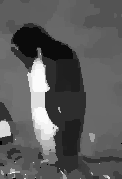
\includegraphics[scale = 0.50]{\imagePath/inpainting_results/penguin_HIER_w40_M40} &
	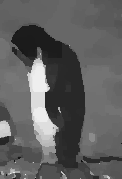
\includegraphics[scale = 0.50]{\imagePath/inpainting_results/confFileInpainting_penguinL20_m1_M40_wc40_labeling} &
	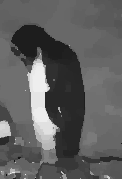
\includegraphics[scale = 0.50]{\imagePath/inpainting_results/confFileInpainting_penguinL20_m3_M40_wc40_labeling} \\
	\scriptsize{(a) Penguin input} & \scriptsize{(b) Cooccurrence} & \scriptsize{(c) Parsimonious} & \scriptsize{(d) $m$ = 1, $L$ = 20} & \scriptsize{(e) $m$ = 3, $L$ = 20}\\
	\scriptsize(Energy, Time (s)) & \scriptsize(14735411, 237) & \scriptsize(12585846, 456) & \scriptsize(12301899, 3962) & \scriptsize($12404499^*$, 5018)\\
	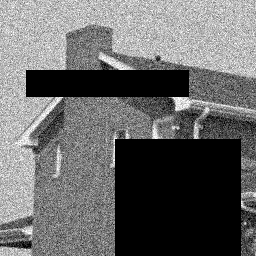
\includegraphics[scale = 0.25]{\imagePath/inpainting_results/house-input} &
	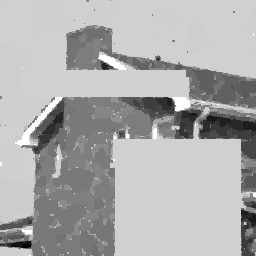
\includegraphics[scale = 0.25]{\imagePath/inpainting_results/house_COOC_w50_M50} &
	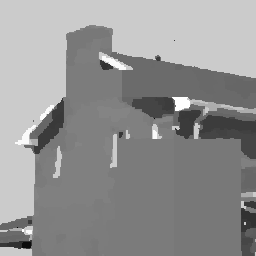
\includegraphics[scale = 0.25]{\imagePath/inpainting_results/house_HIER_w50_M50} &
	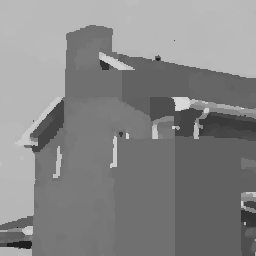
\includegraphics[scale = 0.25]{\imagePath/inpainting_results/confFileInpainting_houseL20_m1_M50_wc50_labeling} &
	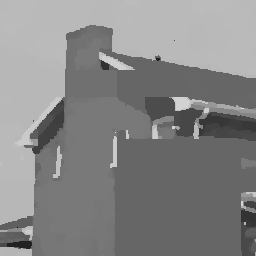
\includegraphics[scale = 0.25]{\imagePath/inpainting_results/confFileInpainting_houseL20_m3_M50_wc50_labeling} \\ 
	\scriptsize(f) House input & \scriptsize(g) Cooccurrence & \scriptsize(h) Parsimonious & \scriptsize(i) $m$ = 1, $L$ = 20 & \scriptsize(j) $m$ = 3, $L$ = 20\\
	\scriptsize(Energy, Time (s)) & \scriptsize(42018464, 486) & \scriptsize(37349032, 12024) & \scriptsize(36903599, 22751) & \scriptsize($37093699^*$, 23260)\\
\end{tabular}
\vspace{2mm}
\mycaption{\footnotesize \em Image inpainting results: Figures (a)  and (f) are input images of `penguin' and `house' respectively with noise and obscured regions. Our results for $m$ = 1 (d) and (i) are significantly better than those of~\cite{ladickyeccv10} (b) and (g) and of~\cite{dokaniaiccv15} (c) and (h)  in terms of energy. We use super-pixels obtained using mean-shift as cliques. Our results preserve details better and look more natural. The baseline results exihit significant blocking effect. $^*$Note that $m$ = 3 uses a different energy function from other cases.}
\label{fig:inpainting_results}
\end{figure}

\myparagraph{\bf Data.} Given an image with noise and obscured/inpainted regions (regions with missing pixels), the task is to denoise it and fill the obscured regions in a way that is consistent with the surrounding regions. The images `house' and `penguin' from the Middlebury data set were used for the experiments. Since the images are grayscale, they have 256 labels in the interval [0, 255], each representing an intensity value. The unary potential for each pixel corresponding to a particular label equals the squared difference between the label and the intensity value at the pixel. We use high-order cliques as the super-pixels obtained using the mean-shift method~\cite{comaniciu2002mean}. The parameters $\omega_c$, $M$ and $m$ are varied to give different truncated max-of-linear energy functions.

\myparagraph{\bf Method.} For each parameter setting of $\omega_c$, $M$ and $m$, we vary the interval lengths for our algorithm and make a comparison with the baselines.

\myparagraph{\bf Results.} Results for $\omega_c$ = 40, $M$ = 40, and $m$ = 1 and 3 for `house' and $\omega_c$ = 50, $M$ = 50, and $m$ = 1 and 3 for `penguin' are shown in Figure~\ref{fig:inpainting_results}. Other results are shown in the supplementary material. In both cases, we used interval length $L$ = 20. Our algorithm consistently gives lower energy labeling as compared to both~\cite{dokaniaiccv15} and~\cite{ladickyeccv10}. For `penguin', our algorithm gives cleaner denoised image, preserving edges and details. On the other hand, both~\cite{dokaniaiccv15} and~\cite{ladickyeccv10} exhibit significant blocking effect. Moreover, the output is more natural for $m$ = 3 as compared to $m$ = 1. Even for `house', our output looks more visually appealing as compared to baselines.


\mysubsubsection{Stereo Matching}

\begin{figure}[t]
	\centering
\begin{tabular}{ccccc}
	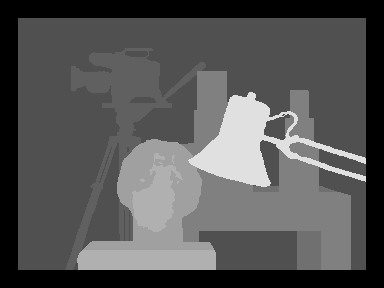
\includegraphics[scale = 0.17]{\imagePath/stereo_results/tsukuba_groundtruth} &
	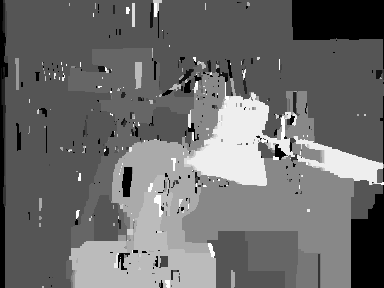
\includegraphics[scale = 0.17]{\imagePath/stereo_results/tsukuba_COOC_M5_wc20} &
	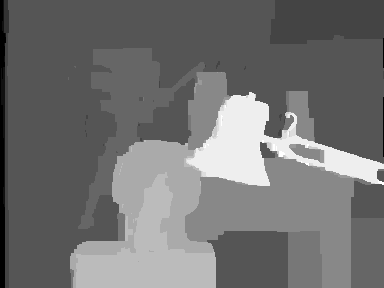
\includegraphics[scale = 0.17]{\imagePath/stereo_results/tsukuba_HIER_M5_wc20} &
	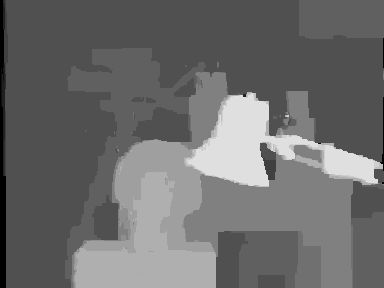
\includegraphics[scale = 0.17]{\imagePath/stereo_results/tsukubaL4_m1_M5_wc20} &
	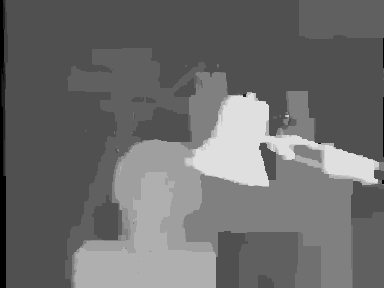
\includegraphics[scale = 0.17]{\imagePath/stereo_results/tsukubaL4_m3_M5_wc20} \\
	\scriptsize(a) Ground truth & \scriptsize(b) Cooccurrence & \scriptsize(c) Parsimonious & \scriptsize(d) $m$ = 1, $L$ = 4 & \scriptsize(e) $m$ = 3, $L$ = 4\\
	\scriptsize(Energy, Time (s)) & \scriptsize(2098800, 101) & \scriptsize(1364200, 225) & \scriptsize(1257249, 256) & \scriptsize($1267449^*$, 335)\\
	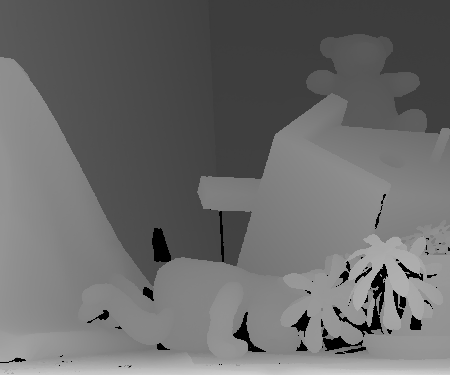
\includegraphics[scale = 0.15]{\imagePath/stereo_results/teddy_groundtruth} &
	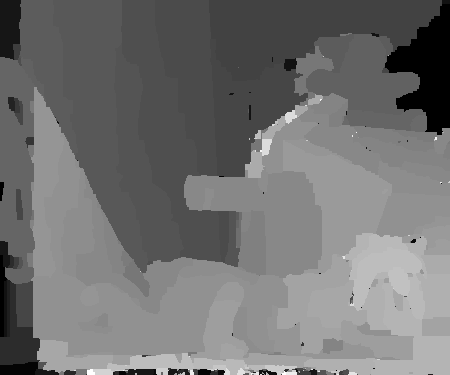
\includegraphics[scale = 0.15]{\imagePath/stereo_results/teddy_COOC_M1_wc20} &
	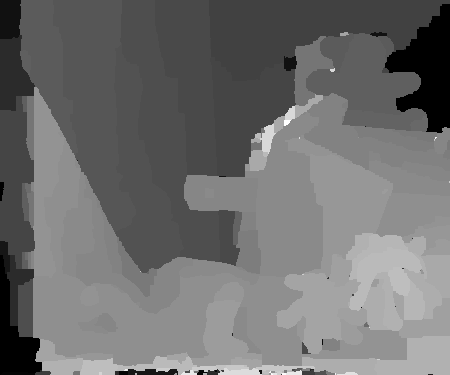
\includegraphics[scale = 0.15]{\imagePath/stereo_results/teddy_HIER_M1_wc20} &
	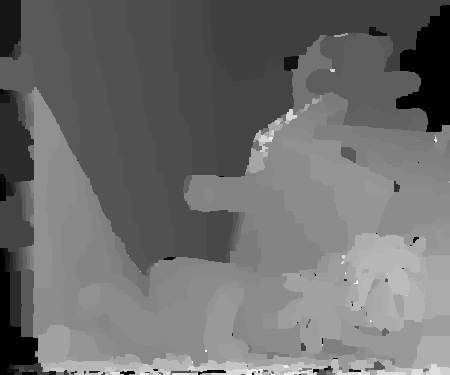
\includegraphics[scale = 0.15]{\imagePath/stereo_results/teddyL1_m1_M1_wc20} &
	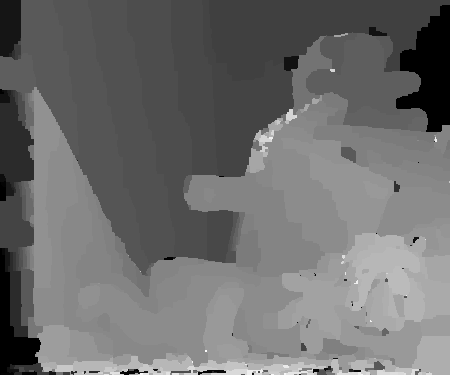
\includegraphics[scale = 0.15]{\imagePath/stereo_results/teddyL1_m3_M1_wc20} \\ 
	\scriptsize(f) Ground truth & \scriptsize(g) Cooccurrence & \scriptsize(h) Parsimonious & \scriptsize(i) $m$ = 1, $L$ = 1 & \scriptsize(j) $m$ = 3, $L$ = 1\\
	\scriptsize(Energy, Time (s)) & \scriptsize(3259900, 495) & \scriptsize(3201300, 484) & \scriptsize(3003949, 1175) & \scriptsize($3015379^*$, 847)\\
	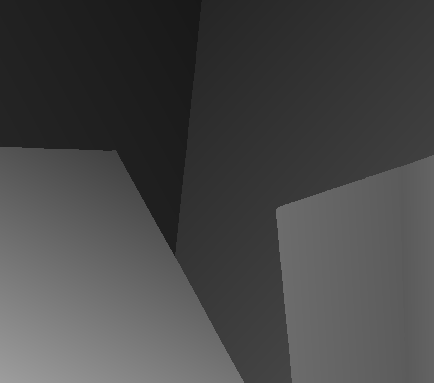
\includegraphics[scale = 0.15]{\imagePath/stereo_results/venus_groundtruth} &
	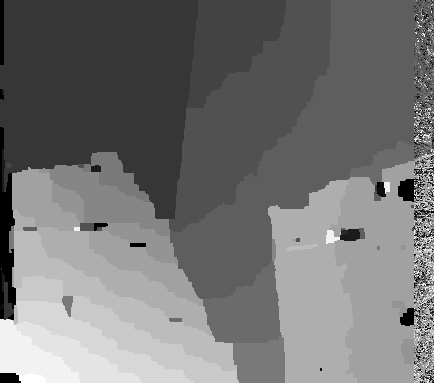
\includegraphics[scale = 0.15]{\imagePath/stereo_results/venus_COOC_M5_wc20} &
	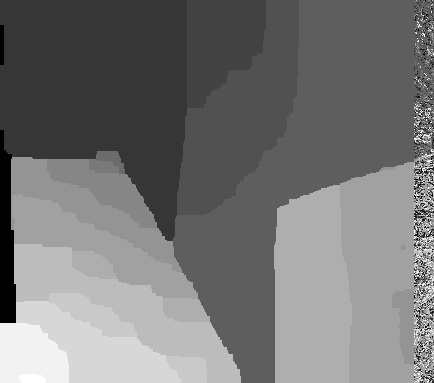
\includegraphics[scale = 0.15]{\imagePath/stereo_results/venus_HIER_M5_wc20} &
	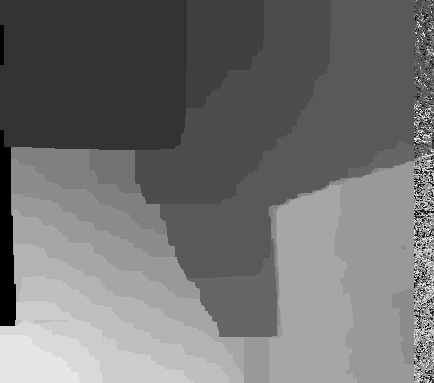
\includegraphics[scale = 0.15]{\imagePath/stereo_results/venusL4_m1_M5_wc20} &
	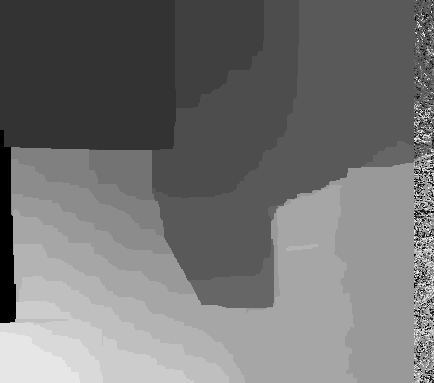
\includegraphics[scale = 0.15]{\imagePath/stereo_results/venusL4_m3_M5_wc20} \\ 
	\scriptsize(k) Ground truth & \scriptsize(l) Cooccurrence & \scriptsize(m) Parsimonious & \scriptsize(n) $m$ = 1, $L$ = 4 & \scriptsize(o) $m$ = 3, $L$ = 4\\
	\scriptsize(Energy, Time (s)) & \scriptsize(2343200, 261) & \scriptsize(2262600, 482) & \scriptsize(2210629, 2700) & \scriptsize($2235689^*$, 3032)\\

\end{tabular}
\vspace{2mm}
\mycaption{\footnotesize \em Stereo matching results: Figures (a), (f) and (k) are the ground truth disparity for `tsukuba', `teddy' and `venus' respectively. Our results for $m$ = 1 (d), (i) and (n) are significantly better than those of~\cite{ladickyeccv10} (b), (g) and (l) and of~\cite{dokaniaiccv15} (c), (h) and (m)  in terms of energy. We also show results for $m$ = 3. We use super-pixels obtained using mean-shift as cliques. $^*$Note that $m$ = 3 uses a different energy function from other cases.}
\label{fig:stereo_matching}
\end{figure}


\myparagraph{\bf Data.} In the stereo matching problem, we have two rectified images of the same scene from two cameras set slightly apart. We are required to estimate the horizontal disparity between a pixel in the right camera image from the corresponding pixel in the left camera. We use `tsukuba' and `teddy' datasets from the Middlebury stereo collection for our experiments. In each case, we have a pair of RGB images and ground truth disparities. We assume the unary potentials to be the $L1$-norm of the difference in RGB values of the left and right image pixels. There are 16 labels and 60 labels for `tsukuba' and `teddy' respectively. The high-order cliques are super-pixels obtained using mean-shift method~\cite{comaniciu2002mean}. The parameters $\omega_c$, $M$ and $m$ are varied to give different truncated max-of-linear energy functions.


\myparagraph{\bf Method.} For each parameter setting of $\omega_c$, $M$ and $m$, we vary the interval lengths for our algorithm and make a comparison with the baselines.

\myparagraph{\bf Results.} Results for $\omega_c$ = 20, $M$ = 5, and $m$ = 1 and 3 for `tsukuba' and `venus', and $\omega_c$ = 20, $M$ = 1, and $m$ = 1 and 3 for `teddy' are shown in Figure~\ref{fig:stereo_matching}. Other results are shown in the supplementary material. We used interval length $L$ as 4 for `tsukuba' and `venus', and 1 for `teddy'. Our algorithm consistently gives lower energy labeling as compared to both~\cite{dokaniaiccv15} and~\cite{ladickyeccv10}. For `tsukuba', our algorithm captures the details of the face better than~\cite{dokaniaiccv15} and~\cite{ladickyeccv10}. For `venus', our algorithm gives smoother labeling for the front plane. Moreover, our results for $m$ = 3 exhibit robustness to inaccurate clique definitions. 

\mysection{Discussion}
We proposed a novel family of high-order random fields called truncated max-of-convex models (TMCM). The energy function of
a TMCM consists of arbitrary unary potentials and high-order clique potentials that are proportional to the sum of the truncation
of the $m$ largest convex distance functions over disjoint pairs of random variables in the clique. In order to enable the use
of TMCM, we developed a novel range expansion algorithm for energy minimization that retains
the efficiency of $st$-{\sc mincut} and provides provably accurate solutions.

From an application point of view, our work opens up the possibility of improving the accuracy of other
computer vision problems such as optical flow and segmentation using TMCM. From a theoretical point of view, our work can be
thought of as a step towards the identification of graph representable submodular functions. We plan to investigate the
properties of the Lov\'{a}sz extension of submodular functions that enables the construction of an equivalent directed graph in
an automated fashion.

\clearpage
{\small
\bibliographystyle{splncs}
\bibliography{eccv2016submission}
}

\end{document}
